\section{K-Means}
\subsection{Implementation}
The added implementation in CPlan \citep{cPlan:2015} is an optimised K-Means version named K-Means++. The idea of this algorithm is to select reasonable start centres to avoid many iterations.

\subsection{Speed Optimization}
The ETH-Zurich provided the following networks: Bad Berka (552 nodes, 626 edges), Weimar (2012 nodes, 2646 edges) and Zurich (27446 nodes, 35121 edges). The network Zurich with factor 13 more edges than Weimar resulted in long processing time. A speed improvement was  achieved by running the K-Means iterations in parallel. Every iteration can be executed free of side effects. The measurements and comparisons of the results are provided in the section Practical Task/Measurements \ref{sec:measurements};

\subsection{Result}
The implementation in CPlan \ref{CPlan} produced the following image \ref{fig:KmeansGenerated} based on the city of Weimar. All streets in one cluster are marked with the same colour, the transitions between clusters are marked black.

\begin{figure}
    \centering
    \begin{mdframed}[style=mdthight]
        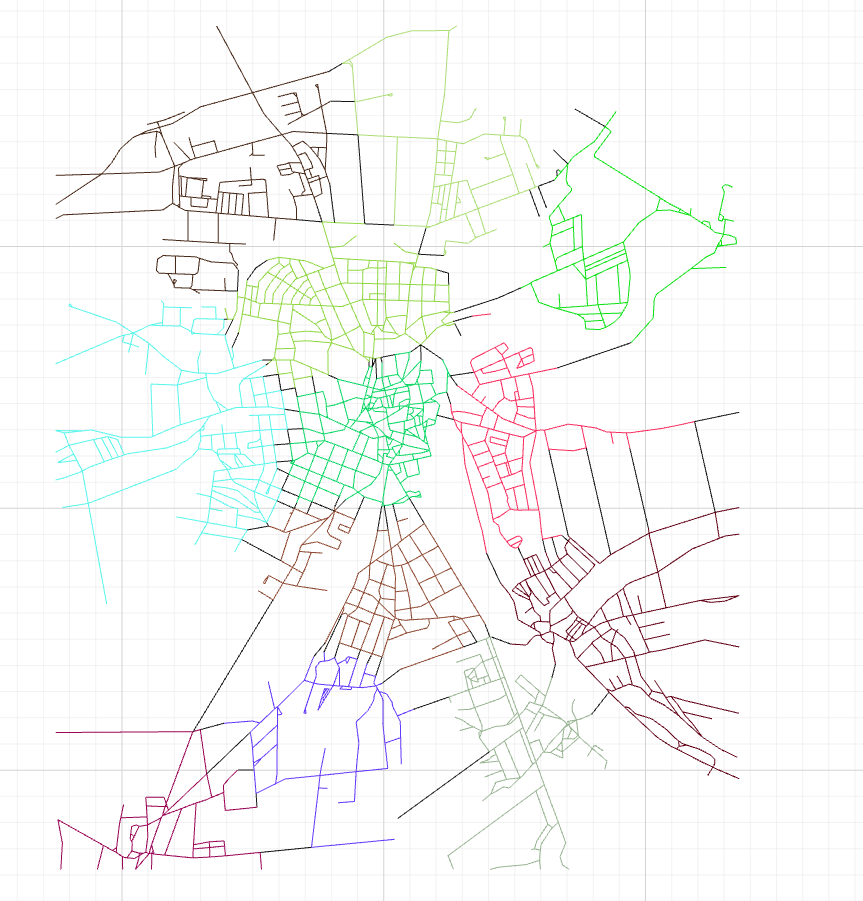
\includegraphics[width=\textwidth]{clusteranalysis_kmeans_result.png}
    \end{mdframed}
    \caption{K-Means cluster analysis of Weimar
    \label{fig:KmeansGenerated}}
\end{figure}

\subsection{Problem} \label{sec:kmenasProblem}
The algorithm is based on the euclidean distance between cluster centroids and street junctions, the edge data (e.g. street length) is not used. As a result it leads to unexpected transitions between clusters. In the image \ref{fig:KmeansProblem} the result can be observed in the read circle where only one point is marked as outer cluster. The two black lines represent the cluster transitions.

\begin{figure}
    \centering
    \begin{mdframed}[style=mdthight, userdefinedwidth=0.55\textwidth, align=center]
        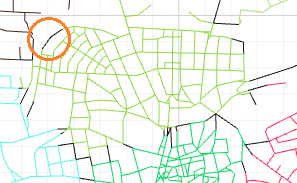
\includegraphics[width=\textwidth]{clusteranalysis_kmeans_problem.png}
    \end{mdframed}
    \caption{Problem of K-Means clustering
        \label{fig:KmeansProblem}}
\end{figure}

\subsection{K-Means with Shortest Path} \label{sec:K-Means_shortest_path}
To solve the problem of unexpected transitions between clusters the best result of the K-Means algorithm can be combined with the distance measurement of a \gls{APSP} algorithm (Dijkstra / Floyd-Warshall). These algorithms are used for the hierarchical clustering algorithms \ref{sec:shortest_path}.

The edges are assigned by the edge data (e.g. street length) to the nearest cluster. Therefore the result is a connected graph. This means every vertex can be reached from every other vertex within a cluster. In the generated figure \ref{fig:Kmeansshortestp} the artefacts described in \ref{sec:kmenasProblem} are removed.

Additional calculation time is needed for the shortest path algorithm. The differences can be compared in the section Measurements \ref{sec:measurements};

\begin{figure}
    \centering
    \begin{mdframed}[style=mdthight]
        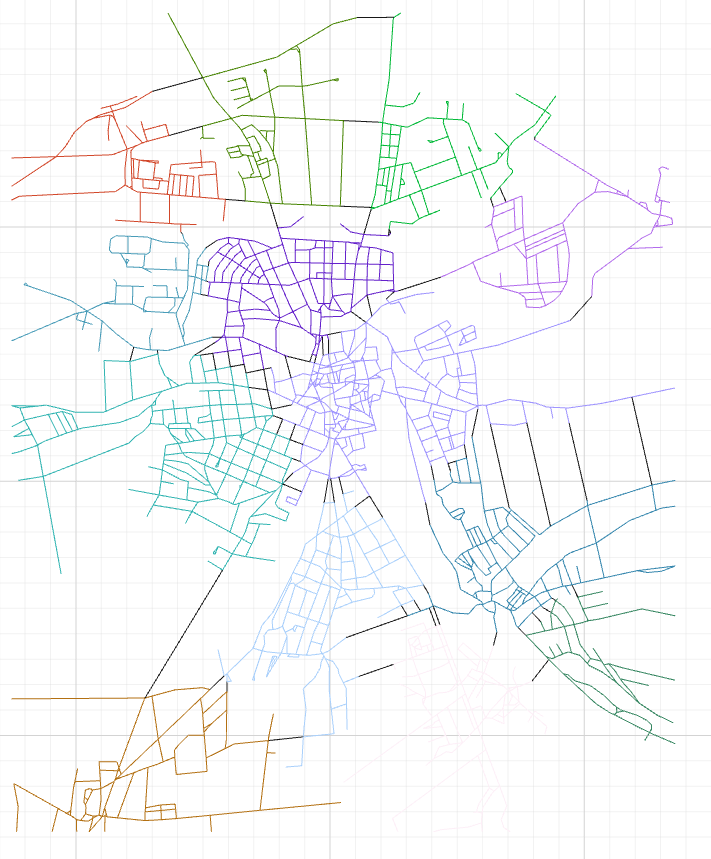
\includegraphics[width=\textwidth]{clusteranalysis_kmeansExt_result.png}
    \end{mdframed}
    \caption{K-Means clustering with shortest path\label{fig:Kmeansshortestp}}
\end{figure}
